\documentclass[journal]{IEEEtran}

%\usepackage[pass,letterpaper]{geometry}              %This package needs to be enaled when dvi--->ps----->PDF
\usepackage{stmaryrd, amsfonts, mathptmx, mathtools, array, siunitx, graphicx,balance,subcaption }
\usepackage{multirow, indentfirst, cite, verbatim, keyval, textcomp, enumerate, calc, microtype, natbib}



\usepackage[colorlinks,linktocpage]{hyperref}
\hypersetup{
   colorlinks   = true,                               %Colours links instead of ugly boxes
   urlcolor     = blue,                               %Colour for external hyper links
   linkcolor    = blue,                               %Colour of internal links
   citecolor    = red,                                %Colour of citations
   setpagesize  = false,
   linktocpage  = true,
}

\IEEEoverridecommandlockouts

\begin{document}
\raggedbottom

\title{\ \\ \LARGE\bf Multi-Agent Based Intellectual Humility Intervention \thanks{}}

\author{Dhanush Bhargav \ Guruksha Gurnani \\ George Washington University}
\markboth{Journal of \LaTeX\ Class Files,~Vol.~xx, No.~xx, May~2025}%
{Shell \MakeLowercase{\textit{et al.}}: Bare Demo of IEEEtran.cls for Journals}
\maketitle

%*********************************************************************************************************************************************************************************************************************
\begin{abstract}
Intellectual humility (IH), the recognition of the limits of one's knowledge and openness to new perspectives, is a crucial trait for constructive discourse. With increasing levels of polarization between individuals, communities, regions, and demographic groups, IH may be more important than ever. This project explores a novel web-based IH intervention that is rooted in established psychological theory and leverages artificial intelligence for scalability and interaction. The intervention protocol is designed to make users consider relevant pieces information about an issue and think about their implications. Multiple large language model (LLM) agents are used to guide each step of the intervention. Post-test IH was significantly higher than IH before the intervention. This work contributes to the young, rapidly-growing fields of intellectual humility and AI-driven interventions, and demonstrates the potential for multi-agent systems to promote cognitive and behavioral change.
\end{abstract}
%*********************************************************************************************************************************************************************************************************************
\section{INRODUCTION}

The advent of internet and especially social media applications has made information more accessible and provided a platform for people to disseminate their views. However, weaponization of information has lead to increased polarization between ideologies, individuals, and communities. This process appears to exacerbate people's tendency to focus on and process content that confirms their initial perceptions and opinions, leading to attitudinal "echo chambers". As a result, open discussion and debate often does not foster broader perspective-taking, but rather increases entrenchment, and in turn, polarization.\\
Intellectual humility (IH) is the recognition of the limits of one's knowledge and openness to new perspectives, and is essential for good judgment and constructive engagement. The intervention protocol explored in this project is designed to provide training in techniques to improve IH by enhancing the awareness and consideration of information relevant to an issue, and generating more-informed responses. This intervention aims to reduce confirmation bias by having participants generate arguments from different sides of various issues, and consider the implications of these arguments for each issue.\\
We utilized large language models (LLMs) to collect, validate, and present arguments as well as prompt participants to consider implications of these arguments. Using LLM agents obviates the need for human mediation and enables greater scalability of the process. This web-based intervention also enables participants to experience and consider others' perspectives while remaining anonymous. The application interface was developed to reflect this goal, offering a structured and intuitive user experience that translates the theoretical steps of the intervention into a smooth, interactive process.
%*********************************************************************************************************************************************************************************************************************
\section{RELATED WORK}
Prior research has established intellectual humility as a critical meta cognitive capacity for recognizing the limits of one’s knowledge and fallibility, with implications spanning leadership, education, and social cohesion. Porter et al.~\cite{porter2022} offers one of the most comprehensive syntheses, arguing that intellectual humility is distinct from related constructs like open-mindedness or modesty because it specifically concerns epistemic limitations. Unlike prior work that often conceptualized humility either as a stable trait or as a fluctuating state, Porter et al.~\cite{porter2022} advocates for a dynamic, context-sensitive view that incorporates both situational variability and cultural influences.
However while Porter et al's.~\cite{porter2022} review extensively catalogs predictors and consequences of intellectual humility, it remains primarily descriptive. Their emphasis lies in mapping the landscape rather than designing mechanisms to foster humility in applied settings. In contrast, our work moves beyond characterization to active intervention: we propose a system designed to operationalize intellectual humility in real-time interactions, adapting to users' conversational cues. Where Porter et al. underscores the challenges posed by personal threat, group dynamics, and cultural contexts in sustaining humility, our approach explicitly addresses these barriers by integrating adaptive dialogue strategies that can reinforce epistemic openness even under conditions of perceived threat or disagreement.
While prior work provides foundational insights into what intellectual humility is and why it matters, our project builds upon these insights to explore \emph{how} it can be practically supported and sustained through technological mediation.
%*********************************************************************************************************************************************************************************************************************
\section{SOLUTION AND METHODOLOGY}
\label{section:solution-methodology}

\subsection{IH INTERVENTION PROTOCOL}
\label{section:ih-intervention-protocol}
\begin{enumerate}
    \item Participants were presented with a central question which can be answered yes/no. The question generally proposed an action or policy decision (e.g., "Should the electoral college be abolished?").
    \item Participants were then asked to choose a stance 'yes' or 'no', followed by how strongly they felt about their stance on a scale of 1 (not at all strongly) to 10 (extremely strongly).
    \item Participants were then asked to consider both sides of the question, and provide as many arguments as they could---with a minimum of one argument for each side.
    \item Participants were then exposed to a larger collection of arguments sourced from other participants, after which they were asked to consider categories into which these arguments could be placed. This step was designed to expose participants to different perspectives.
    \item Next, participants were asked to rate the overall implications of each argument on society as positive, neutral, and negative. Participants were also asked to assess whether---all things considered---the implications of the argument supported the position represented by the question. This step was designed to improve participants' understanding of the extent to which the answer to the central yes/no question makes the outcome represented by each argument better, worse, or neither.
    \item Finally, participants were presented with the central question again, and again asked to indicate their stance and how strongly they felt about it.
\end{enumerate}
\subsection{WEB APPLICATION}
\label{section:web-application}
We developed a web application to provide the intervention protocol to participants and deployed it to the cloud. The application is built around a network of AI-agents, each equipped with tools and instructions to perform specific tasks. The backend is implemented on Python using the CrewAI library for the multi-agent network and hosted in a Flask server.
\begin{figure}
	\begin{center}
		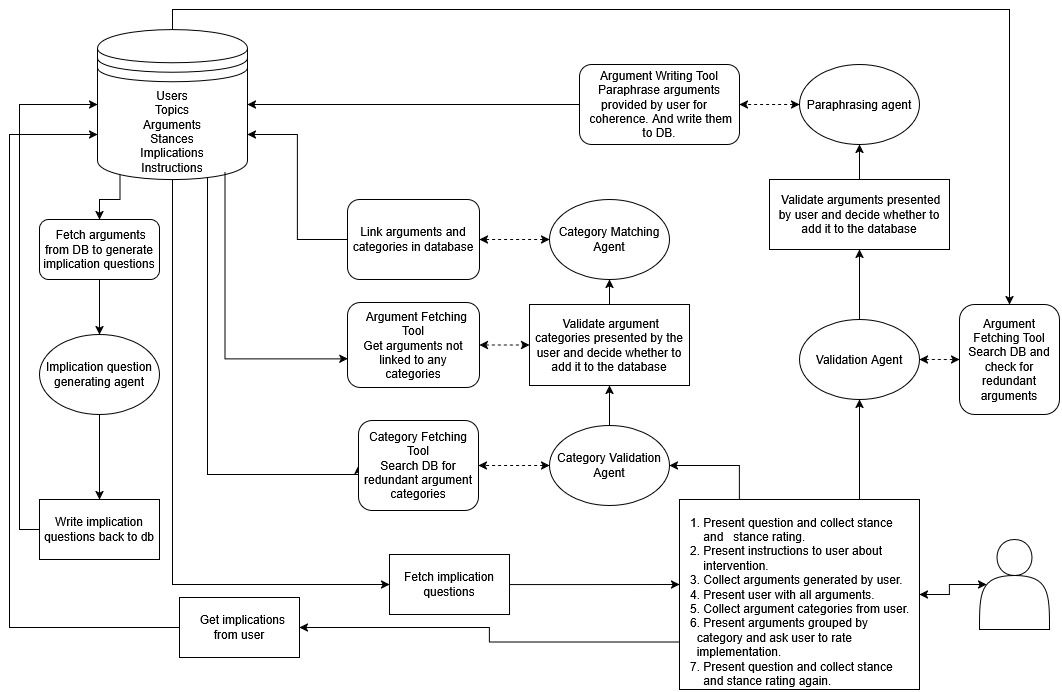
\includegraphics[scale=0.23]{Fig/IHP_architecture.png}
	\end{center}
	\caption{Application architecture showcasing database, AI agents, tools, and user interface}
	\label{figure:application-architecture}
\end{figure}
\subsubsection{BACKEND ARCHITECTURE}
\label{section:backend-architecture}
Figure~\ref{figure:application-architecture} shows the backend architecture of the web application including the database, AI agents, tools and tasks performed by each agent. The key components of the backend are:
\begin{enumerate}
    \item \textbf{Database}: the application used an SQL database with tables to store the users, central questions, arguments, argument categories, implications, along with other data required for the application.
    \item The \textbf{Argument Ingestion Crew} consisted of the \textbf{Validation Agent} and the \textbf{Paraphrasing Agent}. The former was used to validate arguments input by the user for redundancy and relevance while the latter was used to paraphrase the arguments for grammatical correctness and coherence (in case the user's input requires it).
    \item The \textbf{Category Ingestion Crew} consisted of the \textbf{Category Validation Agent} and \textbf{Category Matching Agent}. The former was responsible for validating argument categories provided by the user for redundancy and relevance, while the latter was used to match the arguments to the most appropriate argument categories and to write theese links to the database.
    \item The \textbf{Implication Question Generating Agent} was used to generate implication questions based on each argument and the central topic, which were then saved to the database, and presented to participants.
    \item In addition to the above components, the backend consisted of application programming interfaces (APIs) for logging in, submitting stances, rating implications, and submitting answers to questionnaires.
\end{enumerate}

\subsubsection{USER INTERFACE}
\label{section:user-interface}
The user interface (UI) was developed to operationalize the multistage intervention protocol described in \ref{section:ih-intervention-protocol}. Built using React.js and styled with Material UI, the interface was designed to be responsive, accessible, and easy to navigate, allowing participants to engage meaningfully with each step of the intervention.

After logging in, participants began by completing a series of pre-assessment questionnaires measuring intellectual humility and social desirability. The IH questionnaire consists of 8 questions from \citep{general-intellectual-humility}, and the social desirability questionnaire consists of 11 questions taken from \citep{social-desirability}.

\begin{enumerate}
    \item Participants were then introduced to a central policy question, asked to indicate their position (yes/no), and rated how strongly they felt about their stance on a scale of 1 (not at all strongly) to 10 (extremely strongly).
    \item Participants were then informed about the purpose of the exercise (to help them make more-informed decisions), admonished to try---to the best of their ability---to put aside their opinions about the issue for the duration of the exercise. They were then instructed how to navigate each step of the exercise.
    \item Participants were then instructed to generate as many arguments as they could for both sides of the question, with a minimum of one argument for each side.
    \item These responses were then processed by large language model (LLM) agents that grouped the arguments into thematic categories, while also giving participants the opportunity to suggest additional categories.
    \item Once categorized, participants assessed each argument's impact (positive, neutral, or negative) and evaluated its likelihood if the proposed action were implemented (more likely, less likely, or neutral).
    \item Finally, the central question was again presented to the participants, who were again asked to indicate their stance and the strength of their position. This enabled a test of the intervention's impact on participants' positions vis-\`a-vis the central question.
    \item Participants then repeated steps 2 through 7 for two more central policy questions.
    \item At the end of the intervention, participants completed the IH assessment a second time to assess the intervention's impact on participants' intellectual humility.
\end{enumerate}

\subsubsection{CONTINUOUS DEVELOPMENT}
\label{section:continuous-development}
The web application was continuously improved and development was undertaken to ensure it met usability standards while also implementing the IH protocol accurately. Feedback from stakeholders was sought at every major stage of development to ensure it aligned with their needs and expectations.

The backend went through multiple rounds of development to ensure speed and accuracy, while preventing hallucinations on part of the LLM agents. The UI also underwent many weeks of development to ensure it communicated correctly with the backend, was usable, and easy for users to navigate.

\subsection{DATA COLLECTION}
\label{section:data-collection}
The three central questions selected for this experiment are shown in table \ref{tab:central_questions}. These topics were selected due to their relevance in current times and likelihood of generating diverse perspectives and arguments on both sides (yes/no) of the issue.

\begin{table}[ht]
    \centering
    \begin{tabular}{p{0.15\linewidth}  p{0.65\linewidth}}
        \hline
        \multicolumn{2}{c}{\textbf{Central Questions}} \\
        \hline
        S.No.    & Question \\
        \hline
        1        & Should nuclear power be considered a key part of green energy solutions?\\
        2        & Should universal basic income (UBI) be adopted?            \\
        3        & Should teachers be allowed to carry firearms in schools?             \\
        \hline
    \end{tabular}
    \caption{List of central questions presented to participants.}
    \label{tab:central_questions}
\end{table}

\subsubsection{INITIAL DATA POPULATION}
\label{section:initial-data-population}
To populate the database before opening it up to human participants, we asked AI to generate arguments and argument categories for each of the three questions. We then fed the arguments into the application by following the steps outlined in \ref{section:user-interface}.

\subsubsection{HUMAN PARTICIPATION}
\label{section:human-participation}
Junior and senior university students were selected to participate in this intervention. 
%*********************************************************************************************************************************************************************************************************************
\section{RESULTS AND DISCUSSION}
The data recorded for 48 participants was analyzed to measure the impact of the IH intervention protocol delivered through the web application. The analyses are reported below.

\subsection{CHANGE IN IH SCORE}
Because each question in the IH questionnaire can be answered on a scale of 1(strongly disagree) to 5(strongly agree), the average score over 8 questions was calculated for each participant to assign a single IH score. We then calculate the net change in IH score from the pre-assessment to post-assessment $(\Delta_\text{IH})$ and performed a t-test on the difference from zero of the mean of net changes $(\mu_{\Delta_\text{IH}})$ to test for statistical significance.

\begin{table}[ht]
    \centering
    \begin{tabular}{p{0.15\linewidth}  p{0.65\linewidth}}
\hline
\multicolumn{2}{c}{\textbf{One Sample T-test hypotheses}} \\
\hline
Hypothesis    & Statement \\
\hline
Null $(H_0)$  & Mean of net changes in IH score $(\mu_{\Delta_\text{IH}})$ is not significantly different from zero.\\
Alternate $(H_a)$ & Mean of net changes in IH score $(\mu_{\Delta_\text{IH}})$ is significantly different from zero. \\
\hline
\end{tabular}
    \caption{Null and Alternate Hypotheses for the one-sample t-test on $\mu_{\Delta_\text{IH}}$.}
    \label{tab:hypotheses}
\end{table}

The hypotheses used to perform the one-sample t-test is shown in table \ref{tab:hypotheses} and the results of the test are tabulated in table \ref{tab:ttest-results}.

\begin{table}[ht]
    \centering
    \begin{tabular}{ll}
\hline
\multicolumn{2}{c}{\textbf{One Sample T-test results}} \\
\hline
Statistic    & Value \\
\hline
$\mu_{\Delta_\text{IH}}$  & 0.191 \\
t-statistic & 4.557 \\
p-value & $<.0001$ \\

\hline
\end{tabular}
    \caption{Results for the one-sample t-test on $\mu_{\Delta_\text{IH}}$.}
    \label{tab:ttest-results}
\end{table}

The calculated mean of net changes in IH was $0.191$ $(\text{p}<.0001)$ which is statistically significant with an alpha level of 0.01, two-tailed test. Hence, the null hypothesis stated in table \ref{tab:hypotheses} is rejected. The positive value of $\mu_{\Delta_\text{IH}}$ further indicates that the intervention, on average, led to an increase in IH scores for the participants.

\subsection{STANCE CHANGES REGARDING CENTRAL QUESTIONS}
 To assess stance changes regarding the three central questions, strength ratings (1-10) for all "No" stances were given a negative valence, creating a scale of possible positions from $-10$ (maximally opposed) to $+10$ (maximally supportive). Scatter plots of initial and final stance rating towards the questions in table \ref{tab:central_questions} are shown in Figure \ref{graph:stance-changes-all}. The vertical and horizontal dotted lines divide the graph into 4 quadrants. The points right of the vertical dotted line represent initial "Yes" stances and points to the left represent initial "No" stances. The points above the horizontal dotted line represent final "Yes" stances, and points below it represent final "No" stances. The top right and bottom left quadrants represent participants whose stances remained the same, and the other two quadrants represent participants whose stances changed. 

\begin{figure*}[t!]
    \centering
    \begin{subfigure}[t]{0.3\textwidth}
        \centering
        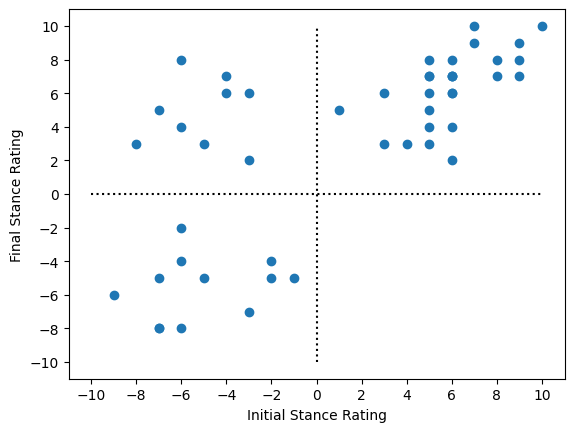
\includegraphics[height=1.5in]{Fig/topic_1_stance_changes.png}
        \caption{Stance changes for question 1.}
        \label{graph:stance-changes-1}
    \end{subfigure}%
    ~
    \begin{subfigure}[t]{0.3\textwidth}
        \centering
        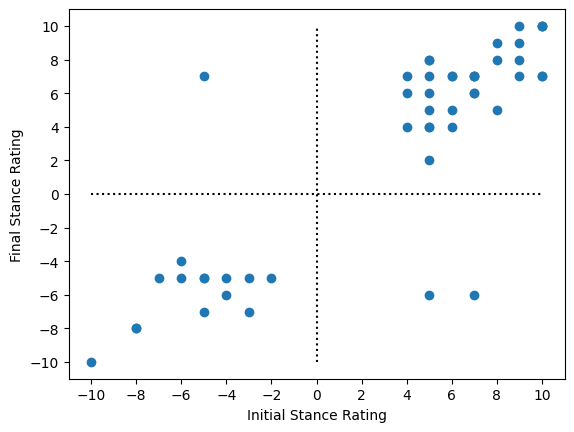
\includegraphics[height=1.5in]{Fig/topic_2_stance_changes.png}
        \caption{Stance changes for question 2.}
        \label{graph:stance-changes-2}
    \end{subfigure}%
    ~
    \begin{subfigure}[t]{0.3\textwidth}
        \centering
        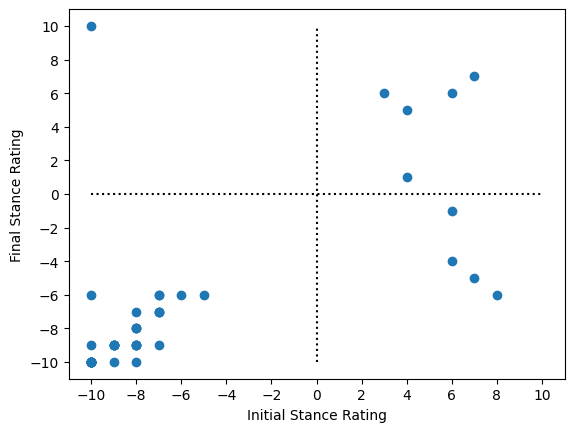
\includegraphics[height=1.5in]{Fig/topic_3_stance_changes.png}
        \caption{Stance changes for question 3.}
        \label{graph:stance-changes-3}
    \end{subfigure}%
    \caption{Stance changes for each of the three central questions.}
    \label{graph:stance-changes-all}
\end{figure*}

As shown in Figure \ref{graph:stance-changes-1} about half of the participants initially opposed to making nuclear power a key energy policy changed their stances after considering the relevant arguments. However, all of those initially in favor of nuclear power remained supportive. About twice as many participants supported as opposed universal income, with only three participants changing their stances (see Figure \ref{graph:stance-changes-2}).  A majority of participants expressed strong opposition---both before and after the intervention---to arming teachers, only one of whom changed their stance, although this change was from maximally negative to maximally positive (see Figure \ref{graph:stance-changes-3}). About half of participants initially in favor of arming teachers ended up opposing this proposition.

\subsection{IMPACT OF SOCIAL DESIRABILITY}
The Social Desirability Scale is designed to assess the importance to participants of being seen by others in a positive light \cite{social-desirability}. It consists of 11 statements (answerable as "yes"(1) or "no"(0)) that reflect either reasonable critical ("I like to gossip at times") or unreasonably positive ("I have never intensely disliked someone") statements about one's self. Responses to the critical items were reverse-coded, and these values were then combined to create a social desirability score between 0 and 11 for each participant, with higher scores reflecting more social desirability.

Since the central topics are designed such that one stance may be perceived as more socially desirable as the other, we need to study the impact of social desirability scores on initial and final stances for each central question.

\begin{figure*}[t!]
    \centering
    \begin{subfigure}[t]{0.3\textwidth}
        \centering
        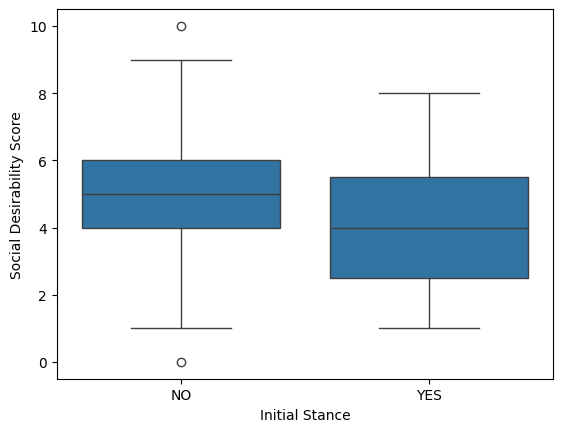
\includegraphics[height=1.5in]{Fig/social_desirability_topic_33.png}
        \caption{Boxplot for question 1.}
        \label{graph:social-desirability-1}
    \end{subfigure}%
    ~
    \begin{subfigure}[t]{0.3\textwidth}
        \centering
        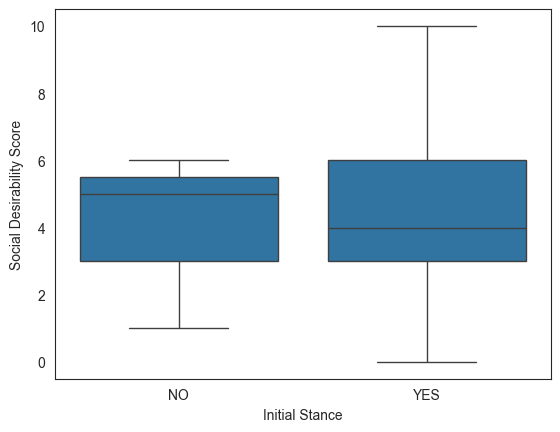
\includegraphics[height=1.5in]{Fig/social_desirability_topic_48.png}
        \caption{Boxplot for question 2.}
        \label{graph:social-desirability-2}
    \end{subfigure}%
    ~
    \begin{subfigure}[t]{0.3\textwidth}
        \centering
        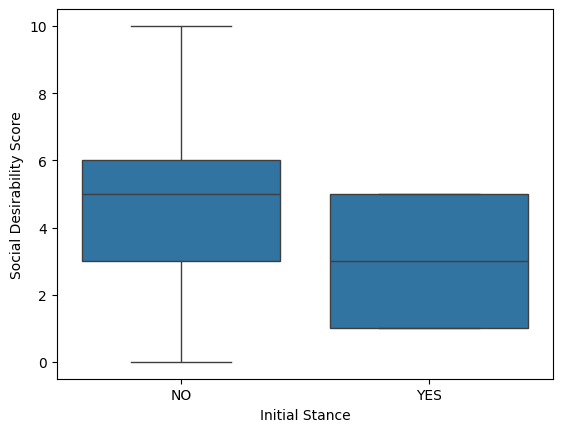
\includegraphics[height=1.5in]{Fig/social_desirability_topic_73.png}
        \caption{Boxplot for question 3.}
        \label{graph:social-desirability-3}
    \end{subfigure}%
    \caption{Box plots of social desirability scores for initial 'yes' and 'no' stances for each central question.}
    \label{graph:social-desirability-all}
\end{figure*}

Figure \ref{graph:social-desirability-all} shows the box-plots of social desirability scores for initial "yes" and "no" responses to all three central topics. We see that for all three central questions, participants who answered "yes" had a lower median social desirability score compared to those who answered "no".

\begin{table}[ht]
    \centering
    \begin{tabular}{ll}
\hline
\multicolumn{2}{c}{\textbf{Two Sample T-test results}} \\
\hline
Topic No.    & p-value \\
\hline
1   &   0.304   \\
2   &   0.880   \\
3   &   0.026   \\
\hline
\end{tabular}
    \caption{Results for the two-sample t-test, comparing means of social desirability scores for initial "yes" and "no" stances for each central question.}
    \label{tab:twosample-ttest-results}
\end{table}

Table \ref{tab:twosample-ttest-results} shows the p-values for the two-sample t-tests that check if the mean social desirability scores are significantly different between participants who took the 'yes' and 'no' stances for each of the three central topics. The p-values for all three tests are higher than the significance level of $0.01$ which indicates that there's no significant difference between mean social desirability scores.

Figure \ref{graph:social-desirability-post-all} shows the box-plots of social desirability scores for final "yes" and "no" responses to all three central topics. We see that for all three central questions, participants who answered "yes" had a lower median social desirability score compared to those who answered "no". However, we perform two-sample t-tests to check if the differences in means are statistically significant.

\begin{figure*}[t!]
    \centering
    \begin{subfigure}[t]{0.3\textwidth}
        \centering
        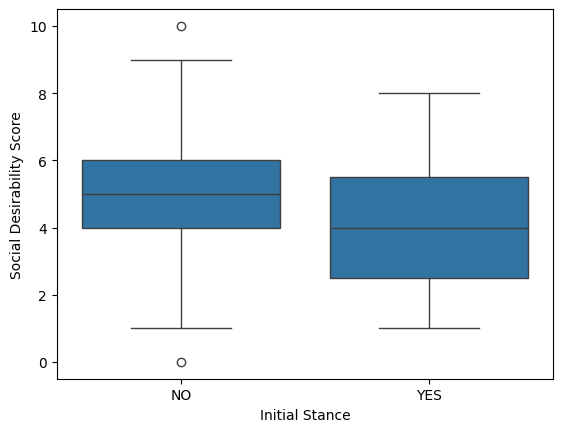
\includegraphics[height=1.5in]{Fig/social_desirability_topic_33.png}
        \caption{Boxplot for question 1.}
        \label{graph:social-desirability-post-1}
    \end{subfigure}%
    ~
    \begin{subfigure}[t]{0.3\textwidth}
        \centering
        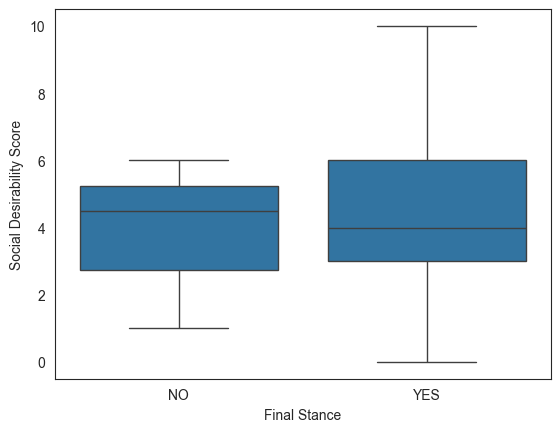
\includegraphics[height=1.5in]{Fig/post_social_desirability_48.png}
        \caption{Boxplot for question 2.}
        \label{graph:social-desirability-post-2}
    \end{subfigure}%
    ~
    \begin{subfigure}[t]{0.3\textwidth}
        \centering
        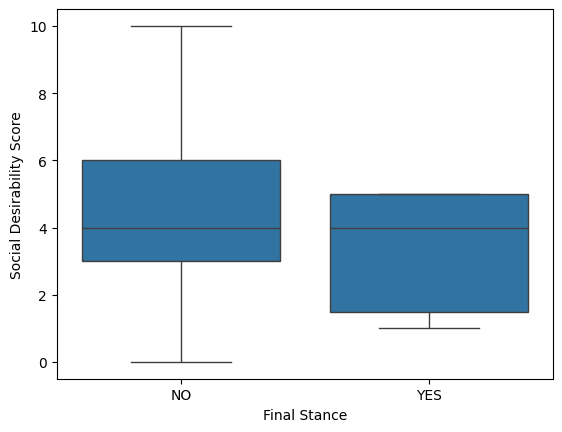
\includegraphics[height=1.5in]{Fig/post_social_desirability_73.png}
        \caption{Boxplot for question 3.}
        \label{graph:social-desirability-post-3}
    \end{subfigure}%
    \caption{Box plots of social desirability scores for final 'yes' and 'no' stances for each central question.}
    \label{graph:social-desirability-post-all}
\end{figure*}

Table \ref{tab:twosample-ttest-post-results} shows the p-values for the two-sample t-tests that check if the mean social desirability scores are significantly different between participants who took the 'yes' and 'no' stances for each of the three central topics. The p-values for all three tests are higher than the significance level of $0.01$ which indicates that there's no significant difference between mean social desirability scores.

\begin{table}[ht]
    \centering
    \begin{tabular}{llr}
\hline
\multicolumn{2}{c}{\textbf{Two Sample T-test results}} \\
\hline
Topic No.    & p-value \\
\hline
1   &   0.718   \\
2   &   0.255   \\
3   &   0.225   \\
\hline
\end{tabular}
    \caption{Results for the two-sample t-test, comparing means of social desirability scores for final "yes" and "no" stances for each central question.}
    \label{tab:twosample-ttest-post-results}
\end{table}

From the two-sample t-tests, we can observe that the social desirability scores of participants does not have a significant impact on their selected stances to the central topics.

%*********************************************************************************************************************************************************************************************************************

\section{CONCLUSION}

This intervention resulted in a significant increase in intellectual humility scores. Because this was a pilot study to check the feasibility and effectiveness of an AI-agent based approach to increase IH, we can conclude that this technique shows promise and warrants further exploration. A/B testing to compare this protocol versus naive methods, and subsequent improvements to the protocol and web application may provide more concrete results about the effectiveness of the approach discussed in this project.

Looking at the initial and final stance and stance ratings, we observe that participants did not typically change stances. However, the aim of this project is not to influence participants' stances on the central topics, but rather to increase the number and implications of arguments they consider then making their judgments. The significant increase in IH suggests that the intervention may well have succeeded in this regard, and that this effect was not due to participants' desire to be viewed in a positive light by others.

%*********************************************************************************************************************************************************************************************************************


\bibliographystyle{IEEEtran}
\balance
\bibliography{mybib}
\end{document}